\section{Analyse}
Nachfolgend werden alle kritischen Elemente der SDA Lösung analysiert. Dazu gehören beispielsweise Dienste, wie die LISP Datenbank, Radius, SGT Access List. und 

Das Ziel ist die komplette Analyse der SDA Lösung und die Identifizierung der kritischen Elemente der Verfügbarkeit (LISP Database, Radius, SGT Access-list etc.) und der Network Services (NTP, DNS, Lizenzen etc.).

\subsection{SDA Architektur und Design}
Die Architektur der Lab Umgebung, welche in der Studienarbeit erarbeitet wurde, sah folgendermassen aus:

\begin{figure}[H]
	\centering
	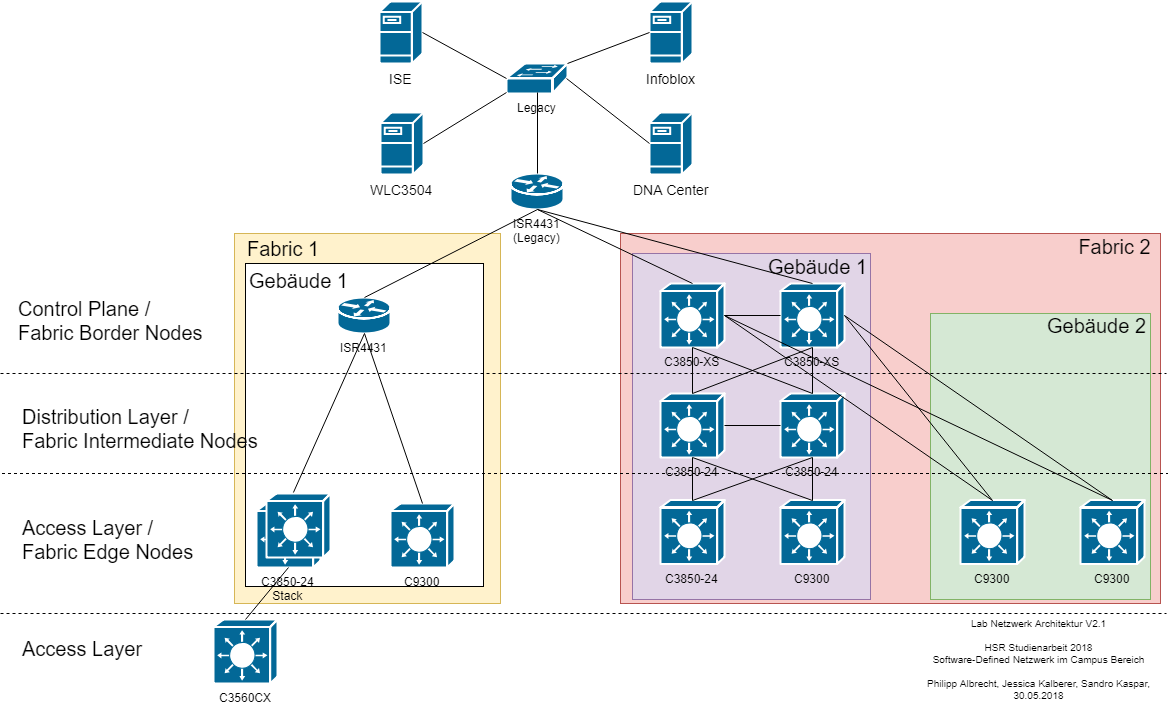
\includegraphics[width=1\linewidth]{img/Architecture/LabNetworkArchitecture_SA}
	\caption{Architektur Studienarbeit}
	\label{fig:Architektur Studienarbeit}
\end{figure}

Die Analyse wird auf dieser Architektur aufbauen und die von der FUB gegebenen Grössenordnung berücksichtigen. \\

Nachfolgend werden die aktuell von Cisco empfohlenen Design Entscheidungen, Grössen\-über\-legungen, sowie die Skalierungen gezeigt. Aktuelle und ausführliche Informationen hierzu, können direkt im SDA Design Guide von Cisco \cite{sda-designguide-sept2018} eingesehen werden. 

\subsubsection{Platform Entscheidungen}
Die Design Entscheidungen beruhen auf den aktuellen Empfehlungen von Cisco, welche sich jedoch laufend ändern können. Nachfolgende Cisco Validated Design (CVD) Empfehlungen sind für die Version 1.2.5 vom September 2018, welche für die zu verwendenden Geräte relevant sind. Ein Catalyst 9300 sollte zum Beispiel nicht als Border oder Control Plane Node verwendet werden. Im Verlauf der Implementation der einzelnen Geräte ist es ausserdem auch wichtig die darauf zu achten, welche genauen IOS Versionen unterstützt werden. 

\begin{figure}[H]
	\centering
	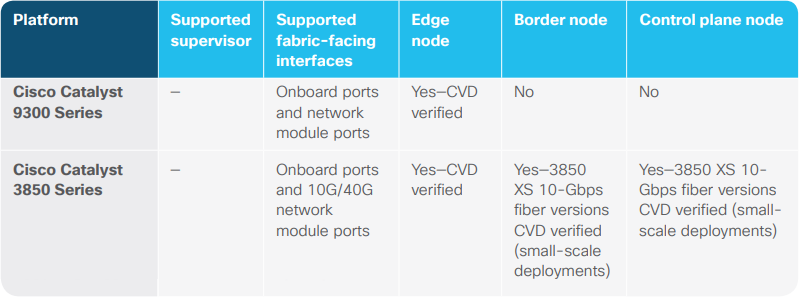
\includegraphics[width=1\linewidth]{img/Analyse/CVD-SDAswitchingplatformsanddeploymentcapabilities-1-2-5}
	\caption{SDA switching platforms and deployment capabilities \cite{sda-designguide-sept2018}}
	\label{fig:SDA switching platforms and deployment capabilities}
\end{figure}

\begin{figure}[H]
	\centering
	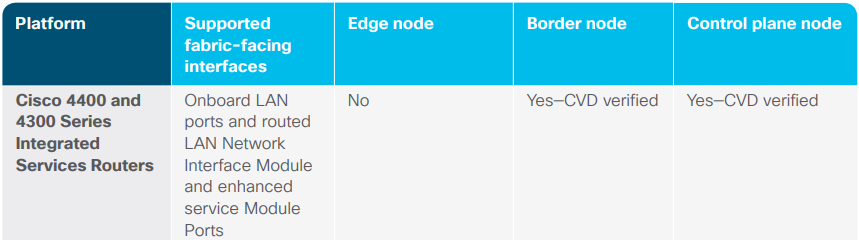
\includegraphics[width=1\linewidth]{img/Analyse/CVD-SDAroutingandwirelessplatformsanddeploymentcapabilities-1-2-5}
	\caption{SDA routing and wireless platforms and deployment capabilities \cite{sda-designguide-sept2018}}
	\label{fig:SDA routing and wireless platforms and deployment capabilities}
\end{figure}

\subsubsection{Grössenüberlegungen}
Diese Grössenüberlegungen sind besonders für grosse Organisationen wichtig, da diese zur Zeit nur bis zu einer gewissen Anzahl von Cisco in der Praxis getestet wurden.


\begin{figure}[H]
	\centering
	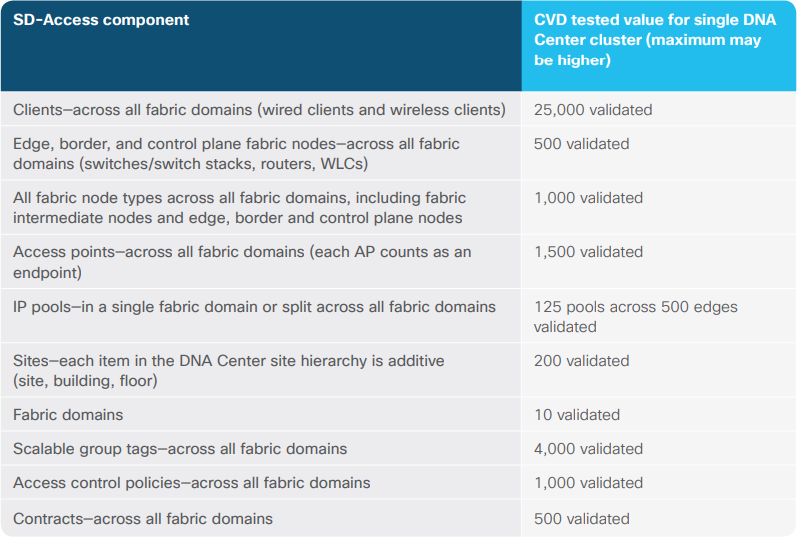
\includegraphics[width=1\linewidth]{img/Analyse/CVD-DNACmanagementofSDA-1-2-5}
	\caption{DNA Center management of SDA \cite{sda-designguide-sept2018}}
	\label{fig:DNA Center management of SDA}
\end{figure}


\begin{figure}[H]
	\centering
	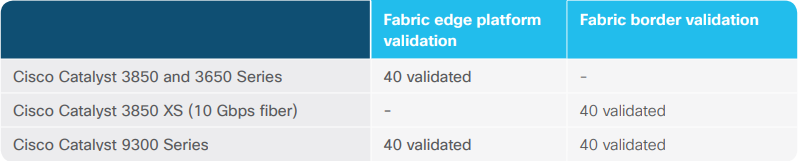
\includegraphics[width=1\linewidth]{img/Analyse/CVD-SDAvirtualnetworksbyplatformandrole-1-2-5}
	\caption{SDA virtual networks by platform and role \cite{sda-designguide-sept2018}}
	\label{fig:SDA virtual networks by platform and role}
\end{figure}


\subsubsection{Maximum Skalierungen}
Folgende maximalen Skalierungen sollten für grosse Organisationen besonders berücksichtigt werden. Diese Daten sollten bei der Auswahl von Plattformen, die während der Planung für das aktuelle und zukünftige Wachstum des Netzwerks verwendet werden, berücksichtigt werden.

Die DNA Center Anzahlen sind pro Instanz, bei denen es sich um ein DNA Center mit einem einzelnen Server oder einem DNA Center Cluster mit drei Servern handeln kann. Die maximalen Zahlen sind entweder die absoluten Grenzen der Plattform oder die empfohlenen Höchstgrenzen aktueller Tests einer einzelnen Plattform.

\begin{figure}[H]
	\centering
	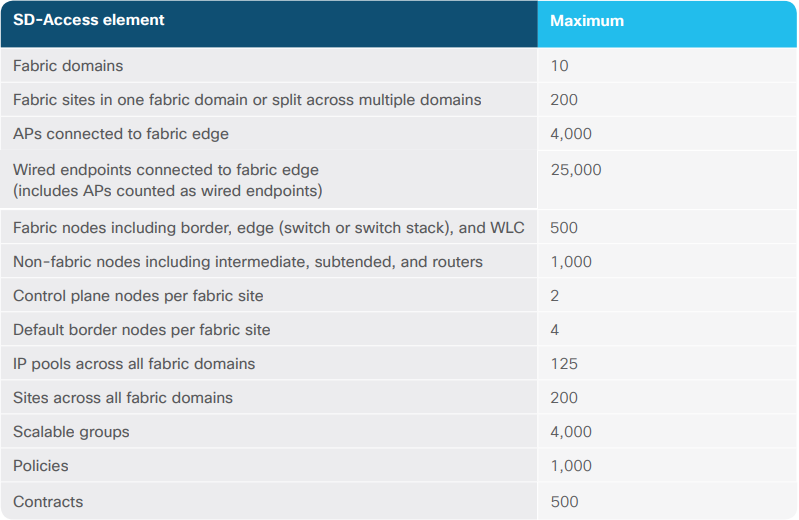
\includegraphics[width=1\linewidth]{img/Analyse/CVD-MaxScale-DNAC-1-2-5}
	\caption{DNA Center Maximum Scale Recommendations \cite{sda-designguide-sept2018} }
	\label{fig:DNA Center Maximum Scale RecommendationsA}
\end{figure}

\begin{figure}[H]
	\centering
	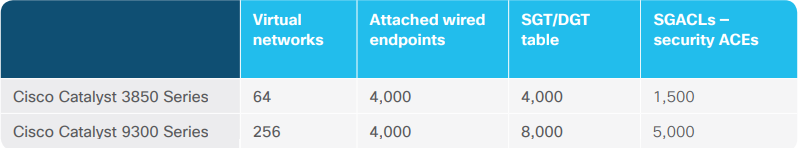
\includegraphics[width=1\linewidth]{img/Analyse/CVD-MaxScale-EdgeNode-1-2-5}
	\caption{Edge Node Maximum Scale Recommendations \cite{sda-designguide-sept2018} }
	\label{fig:Edge Node Maximum Scale RecommendationsA}
\end{figure}

\begin{figure}[H]
	\centering
	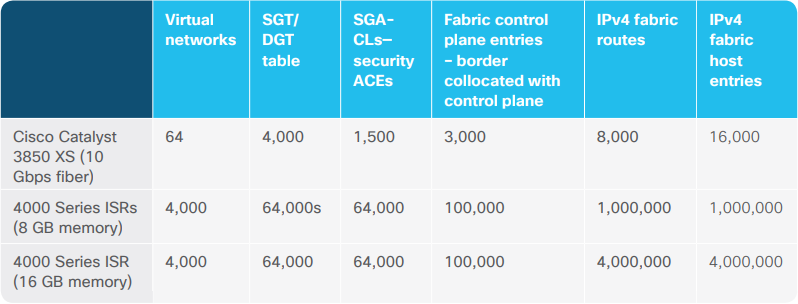
\includegraphics[width=1\linewidth]{img/Analyse/CVD-MaxScale-BorderNode-1-2-5}
	\caption{Border Node Maximum Scale Recommendations \cite{sda-designguide-sept2018} }
	\label{fig:Border Node Maximum Scale RecommendationsA}
\end{figure}



\subsection{Verfügbarkeit}
Die Verfügbarkeit der nachfolgenden Dienste sind für den Betrieb eines SDA mit dem DNA Center wichtig, um die volle Funktion des Netzwerkes bereitstellen zu können. Darum ist es von Vorteil, wenn die kritischen Server und Dienste redundant ausgelegt sind. Den einzelnen Komponenten werden jeweils mit einer Severity (Schweregrad) gewichtet. Die Definitionen der Severities werden von den \textit{Cisco Severity and Escalation Guidelines} übernommen. \cite{cisco-severity-guidelines}

\subsubsection{DNA Center}

\paragraph{Beschreibung}

Das DNA Center übernimmt verschiedene Funktionen im Netzwerk. Es verwaltet die Konfigurationen der Netzwerkgeräte, überwacht diese und stellt die Funktion der Fabrics sicher. 

\paragraph{Impact}

Sollte das DNA Center ausfallen oder nicht erreichbar sein, hat dies keinen direkten Einfluss auf die Funktionalität des Netzwerks. Dies, da alle nötigen Konfigurationen auf den Netzwerkgeräten vorhanden sind. Es ist allerdings nicht mehr möglich, Änderungen am Netzwerk durchzuführen. Es ist beispielsweise nicht mehr möglich, Änderungen an einer Fabric vorzunehmen, Geräte hinzuzufügen oder Access Ports zu konfigurieren. Des Weiteren kann das DNA Center den Betrieb des Netzes nicht mehr monitoren.

\paragraph{Severity} 3

\paragraph{Mögliche Ansätze für mehr Krisenresistenz}

Um die negativen Auswirkungen während eines Ausfalls möglichst gering zu halten, können verschiedene Massnahmen getroffen werden. Dies sind:

\begin{itemize}
\item DNA Center Betrieb im Cluster
\item DNA Center an verschiedenen Standorten
\item Backup, damit schneller Restore möglich ist
\end{itemize}

\subsubsection{LISP Map Server / Control Plane Node}

\paragraph{Beschreibung}

Der LISP Map Server auf dem Control Plane Node verwaltet die RLOCs aller Clients in einer Fabric. Die entsprechenden Edge Nodes melden ihr bekannte Clients an den Control Plane Node, welche diese Information in der LISP Database speichert. Benötigt ein Edge Node die RLOC eines Clients, kann er diesen auf der LISP Database abfragen.

\paragraph{Impact}

Fällt der Control Plane Node aus und die LISP Database steht nicht mehr zur Verfügung, ist die Kommuikation im Netzwerk nur noch eingeschränkt möglich. Clients die sich am selben Edge Node befinden, können weiterhin ohne Einschränkung miteinander kommunizieren. Verbindungen zu Geräten an anderen Edge Nodes sind nur noch möglich, sofern sich diese im Map-Cache des Source Edge Nodes befinden. Dies gilt ebenfalls für Ziele ausserhalb der Fabric, beispielsweise der Internetzugriff.

\paragraph{Severity} 1

\paragraph{Mögliche Ansätze für mehr Krisenresistenz}

Es ist möglich mehrere Control Plane Nodes in einer Fabric zu betreiben. Im DNA Center Release 1.2.5 sind dies bis zu sechs Nodes. Damit kann eine sehr hohe Redundanz gewährleistet werden. Solange mindestens eine Control Plane Node pro Fabric funktioniert, hat der Ausfall der restlichen keinen Einfluss auf den Netzwerkbetrieb. Bei einer Fabric über mehrere Standorte ist es sinnvoll, die LISP Databases dezentral zu positionieren, also über die verschiedenen Standorte zu verteilen, sodass diese lokal noch verfügbar sind, sollte die Kommunikation zum Hauptsitz unterbrochen sein. Ebenfalls ist denkbar, die Map Caches der einzelnen Geräte zu konfigurieren, sodass der letzte funktionierende Stand auch bei einem Ausfall des Map Servers noch auf den Netzwerkgeräten vorhanden ist. 


\subsubsection{ISE / Radius}

\paragraph{Beschreibung}

Die ISE, bzw. ein Radius Server übernimmt alle AAA Aufgaben im Netzwerk. Er ist dafür zuständig, dass sich Clients am Netzwerk authentifizieren können, sowie für die Authentifizierung des DNA Centers auf den Netzwerkgeräten.

\paragraph{Impact}

Fällt dieser Service aus, kann das DNA Center keine Änderungen mehr auf den Devices ausführen. Des Weiteren können sich keine neuen Clients am Netzwerk anmelden. Bereits angemeldete Clients können das Netzwerk solange nutzen, wie Ihre Authentifizierung gültig ist.

\paragraph{Severity} 1

\paragraph{Mögliche Ansätze für mehr Krisenresistenz}

Der Radius Server oder ISE kann redundant betrieben werden. Es können mehrere Instanzen in einem Cluster betrieben werden. Des Weiteren ist eine dezentrale Lösung denkbar. Es kann in Aussenstellen eine Read-Only Kopie des Radius Servers betrieben werden, damit diese autonom funktionieren können, sollte die Verbindung zum Hauptsitz unterbrochen sein.

\subsubsection{SGT Access List}
\paragraph{Beschreibung}
Der Sicherheitsgruppen Tag (SGT) weist jeder Sicherheitsgruppe eine eindeutige 16-Bit-Sicherheitsgruppennummer zu, deren Geltungsbereich in einer TrustSec-Domäne global ist. Die Nummern werden automatisch generiert, wenn eine SGT auf dem ISE erstellt wird. Die Anzahl der Sicherheitsgruppen im Switch ist auf die Anzahl der authentifizierten Netzwerkeinheiten beschränkt.

Die SGT ermöglicht es dem ISE, Richtlinien für die Zugriffssteuerung durchzusetzen, indem es dem Endgerät ermöglicht, auf die SGT zu reagieren, um den Datenverkehr zu filtern.

Die Sicherheitsgruppen-Zugriffssteuerungsliste (SGACL) ermöglicht die Steuerung des Zugriffs und der Berechtigungen basierend auf den zugewiesenen SGTs.

\paragraph{Impact bei Ausfall}
DNA Center: Auf dem DNA Center sind die Sicherheitsgruppen nicht mehr verfügbar und können auch nicht neu erstellt werden.
Netzwerk: Die definierten Policies stehen nicht mehr zur Verfügung. Es werden also nur noch gecachte Policies angewendet, was den Netzwerkbetrieb stark einschränkt. 

\paragraph{Severity} 1

\paragraph{Mögliche Ansätze für bessere Krisenresistenz}
\begin{itemize}
	\item Redundanz des ISE
	\item Read-Only Kopien des ISE / Radius an Aussenstandorten
	\item SGT Access Lists mittels SXP auf alle Nodes statisch deployen (Limitierungen müssen abgeklärt werden)
\end{itemize}

\subsubsection{Border Node}

\paragraph{Beschreibung}

Der Border Node stellt die Verbindung der Fabric zu externen Netzwerken sicher. Unter anderem ermöglicht der Border Node den Internetzugriff.

\paragraph{Impact}

Fallen alle Border Nodes einer Fabric aus, können die Clients der Fabric nur noch innerhalb dieser Fabric kommunizieren. Es ist nicht mehr möglich, mit Devices in anderen Fabrics oder Devices ausserhalb der Fabrics, bzw. dem Internet zu kommunizieren.

\paragraph{Severity} 2

\paragraph{Mögliche Ansätze für mehr Krisenresistenz}

Es können pro Fabric maximal zwei Border Nodes definiert werden. Damit kann eine Redundanz sichergestellt werden, sodass beim Ausfall eines Nodes keine Einschränkungen für die Clients entstehen. 

\subsubsection{Fusion Router}

\paragraph{Beschreibung}

Der Fusion Router stellt die Kommunikation zwischen den verschiedenen Fabrics, sowie zwischen den Fabrics und der Aussenwelt sicher. Dies ist somit eine sehr zentrale Komponente, die für den Betrieb des Netzwerks sehr wichtig ist.

\paragraph{Impact}

Fällt der Fusion Router aus, ist keine Kommunikation zwischen verschiedenen Fabrics mehr möglich. Ebenfalls sind die Verbindungen zu Legacy Netzwerken und dem Internet unterbrochen. Dies kann einen sehr grossen Einfluss haben, da sich DNA Center, ISE und weitere zentrale Komponenten in Legacy Netzwerken befinden können.

\paragraph{Severity} 2

\paragraph{Mögliche Ansätze für mehr Krisenresistenz}

Der Fusion Router sollte redundant vorhanden sein. Dabei ist zu beachten, dass die Border Nodes dann Verbindungen zu allen Fusion Routern haben sollten.

\subsubsection{DHCP}

\paragraph{Beschreibung}

Der DHCP Service, in der Lab Umgebung ist dies Infoblox, stellt sicher, dass die Clients im Netzwerk die korrekten IP Adressen erhalten.

\paragraph{Impact}

Fällt der DHCP Service aus, erhalten neue Clients keine IP Adressen mehr. Die Netzwerkkommunikation ist für diese daher unmöglich. Bestehende Clients können ihre bereits bezogene IP Adresse weiter verwenden, bis die Lease Time abgelaufen ist. Danach sind auch diese Clients offline.

\paragraph{Severity} 2

\paragraph{Mögliche Ansätze für mehr Krisenresistenz}

Infoblox kann als High-Availability Cluster mit zwei Nodes betrieben werden. Damit ist die nötige Redundanz gegeben, sodass ein Node ohne Impact ausfallen kann. Mit dem DNA Center können für Aussenstandorte separate DHCP Server konfiguriert werden, sodass diese bei einem Unterbruch zum Hauptsitz autonom funktionieren können.


\subsubsection{NTP}
\paragraph{Beschreibung}
Das Network Time Protocol (NTP) ist ein Standard zur Synchronisierung der Zeit auf den verschiedenen Systemen.

\paragraph{Impact bei Ausfall}
Bei einem Ausfall des NTP Services kann es zu Problemen bei der Validierung von Zertifikaten kommen. Zudem können auf Grund von falschen Zeiten Events oder Logeinträge fehlerhaft generiert werden. Dies kann eine spätere Fehlersuche stark erschweren.

\paragraph{Severity} 3

\paragraph{Mögliche Ansätze für bessere Krisenresistenz}
Es können mehrere NTP Server unabhängig voneinander betrieben werden. Um eine möglichst genaue Zeit zu erreichen, ist es sinnvoll, an jedem Standort eigene NTP Server zu haben.

\subsubsection{DNS}
\paragraph{Beschreibung}
Das Domain Name System (DNS) ist eine wesentliche und oft unterschätzte Komponente in einem Netzwerk. Es ist wichtig, dass DNS im Netzwerk korrekt funktioniert und jederzeit zur Verfügung steht.

\paragraph{Impact bei Ausfall}
Namensauflösung der Geräte funktioniert nicht mehr. Dies kann dazu führen, dass Services und Geräte nicht mehr erreichbar sind, sofern der Zugriff über Domainnamen und nicht über IPs funktioniert.

\paragraph{Severity} 1

\paragraph{Mögliche Ansätze für bessere Krisenresistenz}
\begin{itemize}
	\item Redundante DNS Server im Infoblox HA Cluster
	\item Read-Only DNS Server an Aussenstandorten zum Beispiel mittels Zone Transfer
\end{itemize}

\subsubsection{Lizenzen}
\paragraph{Beschreibung}
Die Lizenzen der Geräte können über das DNA Center verwaltet werden. Dazu ist jedoch ein Cisco Smart Account nötig, der über alle Lizenzen verfügt. Sind die Lizenzen einmal auf dem DNA Center synchronisiert und ersichtlich, so muss keine Internetverbindung bestehen, da kein Lizenzenforcement besteht.

Die Lizenzen für die einzelnen Switches müssen beim Kauf unbedingt beachtet werden.

\paragraph{Impact bei Ausfall}
Keine, da Lizenzen nicht enforced werden und Lizenzen somit weiterlaufen.

\paragraph{Severity} 4

\paragraph{Mögliche Ansätze für bessere Krisenresistenz}
Richtige Lizenzen für alle Geräte von Anfang an einplanen.

\subsubsection{Hardware}
\paragraph{Beschreibung}
Bei der Hardware handelt es sich, abhängig vom Dienst der darauf bereitgestellt wird, um eines der wichtigsten Komponenten. Läuft die Hardware nicht mehr, so können auch die Dienste welche darauf laufen nicht mehr ausgeführt werden. 

\paragraph{Impact bei Ausfall}
DNA Center, ISE, Netzwerk nicht mehr verfügbar

\paragraph{Severity} Abhängig von der Komponente

\paragraph{Mögliche Ansätze für bessere Krisenresistenz}
Bei der Hardware ist zu beachten, dass sowohl der Strom, als auch die Netzwerkverbindungen redundant vorhanden sind. Ebenfalls sollte die Hardware bei einem Stromausfall durch eine USV eine gewisse Zeit weiter betrieben werden können. Ein Backup für den Notfall ist immer zu empfehlen, damit bei einem Hardwaredefekt ein schneller Restore möglich ist. Ersatzgeräte sind von Vorteil.

\paragraph{Wireless Controller}
\paragraph{Beschreibung}
Der Wireless Controller managed die Access Points und stellt den Betrieb des Wireless LAN sicher. Da Wireless aber kein Bestandteil dieser Arbeit ist, wird nicht genauer darauf eingegangen.

\paragraph{Impact bei Ausfall}
Bei einem Ausfall aller WLCs stehen keine Wireless Netzwerke mehr zur Verfügung. Die Kommunikation für drahtlose Clients ist somit nicht mehr möglich.

\paragraph{Severity} 2

\paragraph{Mögliche Ansätze für bessere Krisenresistenz}
\begin{itemize}
	\item Wireless Controller redundant auslegen
	\item Ersatzgeräte bereithalten
\end{itemize}
